\documentclass[11pt,letterpaper]{article}

% --------------------------------------------------
% PAQUETES
% --------------------------------------------------

\usepackage[utf8]{inputenc}
\usepackage[T1]{fontenc}
\usepackage[spanish]{babel}

\usepackage{amsmath}
\usepackage{amssymb}
\usepackage{amsfonts}

\usepackage{graphicx}
\usepackage{float}
\usepackage{booktabs}

\usepackage{geometry}
\usepackage{fancyhdr}
\usepackage{setspace}

\usepackage{caption}
\usepackage{multirow}
\usepackage{xcolor}
\usepackage{csquotes} % Para citas textuales

\DeclareMathOperator{\arcsec}{arcsec}

% --------------------------------------------------
% CONFIGURACIÓN DE PÁGINA
% --------------------------------------------------

\geometry{
    letterpaper,
    left=2.5cm,
    right=2.5cm,
    top=2.5cm,
    bottom=2.5cm
}

% Interlineado
\onehalfspacing

% Solución al warning de fancyhdr
\setlength{\headheight}{14pt}

% --------------------------------------------------
% ENCABEZADO Y PIE DE PÁGINA
% --------------------------------------------------

\pagestyle{fancy}
\fancyhf{}

\lhead{Astronomía Estelar}
\rhead{Benjamín Collao}

\cfoot{\thepage}

% --------------------------------------------------
% DATOS DEL DOCUMENTO
% --------------------------------------------------

\title{\textbf{Astronomía Estelar}}
\author{Benjamín Collao}
\date{\today}

\begin{document}

\maketitle

\section{Índice}
\begin{itemize}
    \item Introducción: ¿Qué es una estrella?
    \item Unidad 1: Ecuaciones de estructura
    \item Unidad 2: Procesos radiativos
    \item Unidad 3: Procesos nucleares
    \item Unidad 4: Equilibrio e inestabilidad
    \item Unidad 5: Evolución estelar 
    \item Unidad 6: Evolución estelar II, remanentes estelares
\end{itemize}

\section{Introducción}

Las estrellas son, en esencia:
\begin{itemize}
    \item Cuerpos esféricos compuestos principalmente por \textbf{hidrógeno}
    \item Se encuentran en \textbf{equilibrio hidrostático} entre su propia \textbf{gravedad} y \textbf{presión interna}
    \item \textbf{Pierden energía por radiación} desde su superficie, esto implica generalmente la presencia de una \textbf{fuente de energía central} (proporcionada por reacciones de \textbf{fusión nuclear}), que distingue a las estrellas de otros cuerpos. 
    esta es normalmente \textbf{autorregulada} (más energía $\to$ expansión $\to$ enfriamiento).
    \item Los procesos radiativos dependen de la \textbf{composición química} de la estrella.
\end{itemize}

Se entiende por lo menos desde el siglo XVII que las estrellas son ``soles lejanos''. Sin embargo, se comprende su estructura interna solo desde el siglo pasado. Las propiedades principales de las estrellas que se pueden observar directamente o medir fácilmente son, en orden histórico:

\begin{enumerate}
    \renewcommand{\labelenumi}{\Roman{enumi}.}
    \item La \textbf{luminosidad aparente} es la propiedad medible más básica. El primer esquema de clasificación por brillo que conocemos es el de Hiparco (II AC), que dividió las estrellas en seis categorías de ``tamaño'' llamadas \textbf{magnitudes} $m$, con las estrellas más brillantes en la primera categoría ($m=1$) y las más débiles en sexta ($m=6$). Debido a las características del ojo humano, la escala de magnitudes de Hiparco corresponde a una \textbf{progresión logarítmica en brillo}, con una diferencia de 1 mag correspondiente a un factor $\sim 2x$ en brillo. Por esta razón, este tipo de escala logarítmica se encuentra en otros esquemas antiguos de clasificación estelar (p.ej., Fig. 1: magnitudes estelares codificadas como tamaño/área en viejos mapas estelares coreanos).
    
    \begin{figure}[H]
        \centering
        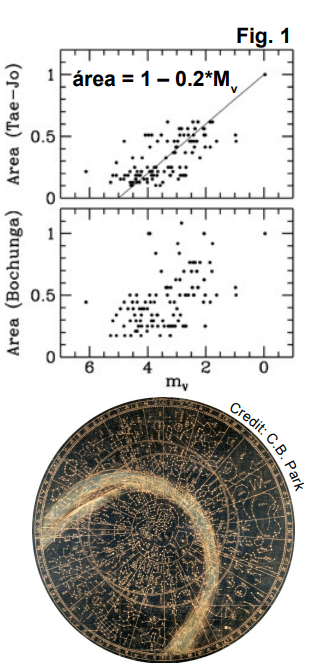
\includegraphics[width=0.3\textwidth]{imagenes/fig 1.png}
        \caption{Magnitudes estelares en mapas antiguos.}
        \label{fig:fig1}
    \end{figure}    
    
    La definición moderna de la \textbf{magnitud} de un objeto con \textbf{densidad de flujo radiativo} (brillo aparente) $f$ como
    \begin{equation}
        m = -2.5 \log_{10}\left(\frac{f}{Q_{ref}}\right)
    \end{equation}
    donde $Q_{ref}$ es una constante de normalización, que define un \textbf{sistema de magnitudes.} Los dos sistemas más comúnmente utilizados hoy son:
        \begin{itemize}
            \item El sistema \textbf{Vega} usa la estrella Vega (o $\alpha$ Lyrae) como referencia. Su espectro tiene la ventaja de ser más fácil de medir y suave en el rango visible. En este sistema, $Q_{ref}$ cambia con la longitud de onda.
            \item El sistema \textbf{monocromático AB}, donde la normalización es \textbf{constante con la frecuencia: $m_v = -2.5\log_{10}f_v - 48.59.$} 
        \end{itemize}
    En general, los puntos cero de los sistemas de magnitud como AB son configurados para coincidir con el sistema Vega de la banda visible (V).
    Por ejemplo, \textbf{$m_{V,Vega}=m_{V,AB}$}.
    
    \item La \textbf{distancia} se obtiene típicamente por mediciones de \textbf{paralaje $p$}, es decir, el \textbf{medio ángulo} entre las posiciones aparentes de un objeto distante, medidas desde \textbf{lados opuestos de la órbita terrestre} (es decir, a un intervalo de 6 meses). Por lo tanto la \textbf{distancia trigonométrica} del objeto es:
    \begin{equation}
        d = \frac{1 AU}{\tan (p)} \approx \frac{1}{p} AU
    \end{equation}
    con $p$ en radianes.
    A partir de esto podemos definir una unidad de distancia llamada \textbf{parsec} (para ``paralaje segundo''), que corresponde al caso de \textbf{$p = 1''$}: $d = \frac{1}{p / \arcsec} pc$ , con 1 pc $\approx$ 3.262 años luz.
    El paralaje de las estrellas más cercanas es significativamente más pequeño (>60 veces) que la \textbf{resolución} angular del \textbf{ojo humano (1 arcmin).} Consecuentemente no se pudo medir antes de la invención del \textbf{telescopio.}
    De hecho la primera medición exitosa de un paralaje estelar fue llevada a cabo por Friedrich Bessel solo en 1838, para la estrella \textbf{61 Cygni} ($p \approx 0.286'', d \approx 11.4 ly, o 3.5 pc$). Por comparación el telescopio astrométrico más moderno, la sonda espacial \textbf{Gaia}, alcanza una precisión de $0.00002''$ $(20 \mu as)$ y puede por lo tanto medir paralajes estelares con un error de menos del $10\%$ hasta el centro de la Vía Láctea, a una distancia de unos 30'000 ly.

    \begin{figure}[H]
        \centering
        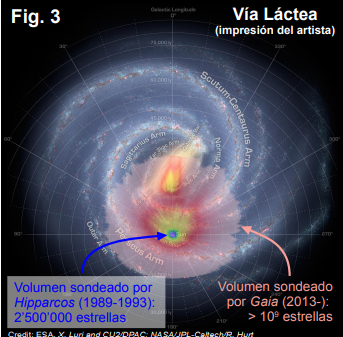
\includegraphics[width=0.3\textwidth]{imagenes/fig 2.png}
        \caption{Paralaje estelar.}
        \label{fig:fig2}
    \end{figure}
    
    Conocer la distancia de una estrella nos permite definir su \textbf{magnitud absoluta}, es decir, su magnitud aparente vista a una distancia de 10 pc: $M = m + 5 (\log_{10}(\frac{d}{pc})-1)$ 
    Por ejemplo, la magnitud visual aparente del Sol desde la Tierra es de -26,74, pero su magnitud absoluta solo 4.72.
    
    \item \textbf{Temperatura:} Al primer orden, la emisión de luz de las estrellas es aproximadamente la de un \textbf{cuerpo negro} (Fig. 2)
    
    \noindent
    \begin{minipage}{0.35\textwidth}
        \centering
        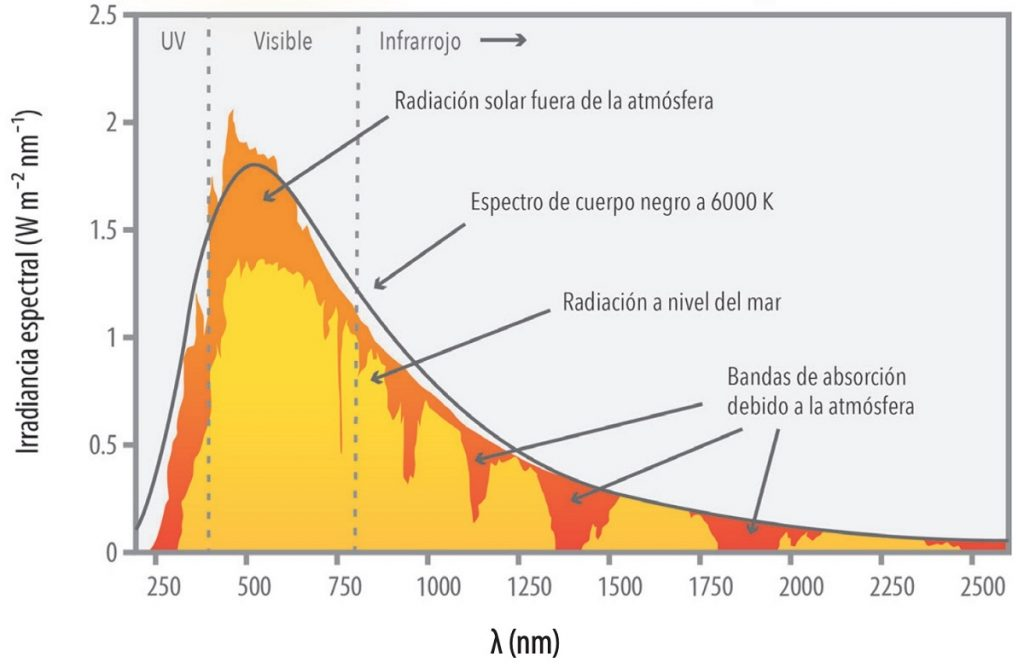
\includegraphics[width=\textwidth]{imagenes/fig 3.jpg}
        \captionof{figure}{Espectro del sol}
        \label{fig:fig3}
    \end{minipage}
    \hfill
    \begin{minipage}{0.60\textwidth}
        \begin{equation}
            F_{\lambda}(T)=\frac{2hc^2}{\lambda^5}(e^{hc/\lambda k_BT}- 1)^{-1}
        \end{equation}
        con la máxima energía emitida a una longitud de onda dada por la \textbf{ley de desplazamiento de Wien}:
        \begin{equation}
            \lambda_{max} =\frac{3\times10^7}{T/k_B}
        \end{equation}
        Según la ley de Stefan-Boltzmann, la luminosidad $L_S$ de una estrella es por lo tanto $L_S=4\pi {R_S}^2 \int F_{\lambda}d\lambda = 4 \pi {R_S}^2 \sigma {T_{eff}}^4$, donde $R_S$ es su radio y $T_{eff}$ su \textbf{temperatura efectiva}. Esta se puede entonces determinar:
    \end{minipage}
    
    \begin{itemize}
        \item Directamente, conociendo $L_S$ y $R_S$
        \item Con modelos de atmósferas estelares
    \end{itemize}
    
    \begin{figure}[H]
        \centering
        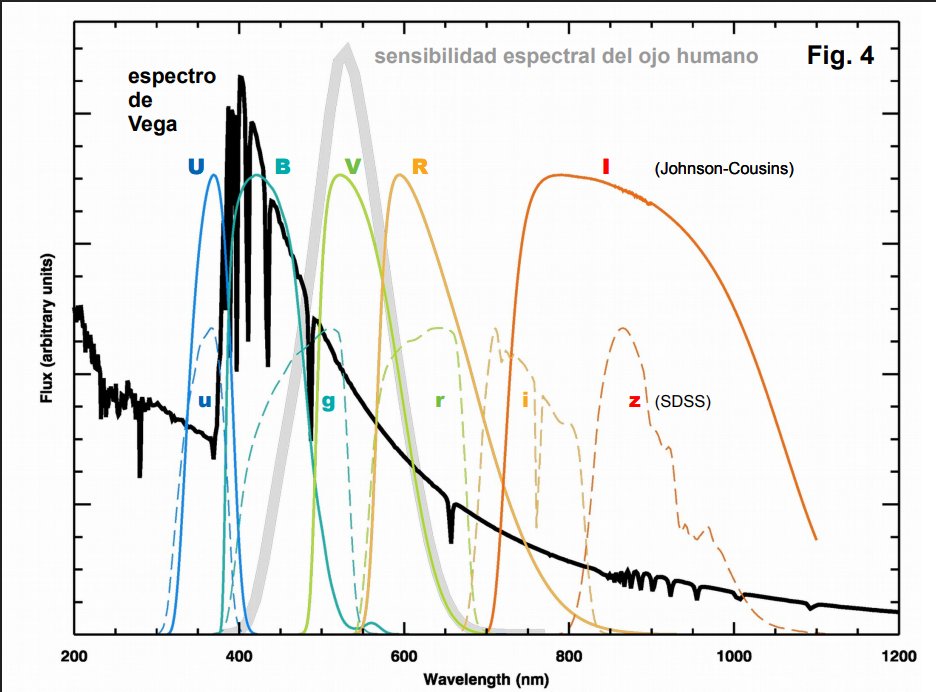
\includegraphics[width=0.5\textwidth]{imagenes/fig 4.png}
        \caption{Descripción de la figura}
        \label{fig:fig4}
    \end{figure}
    
    \begin{itemize}
        \item Por índices \textbf{color}, es decir, un muestreo de la emisión de la estrella usando \textbf{filtros fotométricos.} El primer sistema de filtros fotométricos fue el sistema \textbf{UBVRI} de \textbf{Johnson}-Cousins (Fig. 4: Ultraviolet, Blue, Visual, Red, Infrared). La densidad de flujo $f_{\lambda ,i}$ de una fuente con espectro $F_{\lambda}$ a través de un filtro $i$ con una respuesta espectral $R_i$ es entonces:
    \end{itemize}
    \begin{equation}
        f_{\lambda ,i} = \frac{\int F_{\lambda}(\lambda)R_i(\lambda)\lambda d\lambda}{\int R_i \lambda d\lambda}
    \end{equation}
    
    \begin{figure}[H]
        \centering
        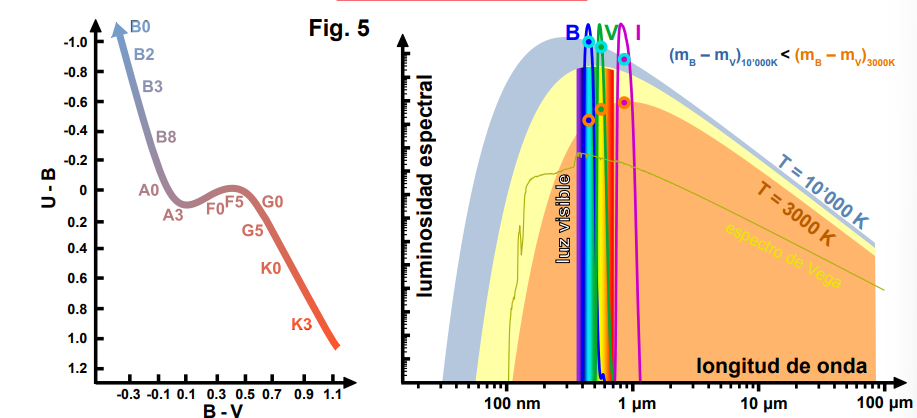
\includegraphics[width=0.8\textwidth]{imagenes/fig 5.png}
        \caption{Filtros fotométricos.}
        \label{fig:fig5}
    \end{figure}
    
    Para un detector de conteo de fotones (de ahí el $\lambda$ suplementario, la tasa de fotones siendo $F_{\lambda}*\lambda / hc$, ya que la energía de los fotones es $hv$, $vF_v=\lambda F_{\lambda}$ y $\lambda v = c$). Un \textbf{color fotométrico} se define entonces como la diferencia de magnitud entre los dos filtros, por ejemplo:
    \begin{equation}
        m_i - m_j = -2.5\log (f_i/f_j) + z_{ij}
    \end{equation}
    Donde $z_{ij}$ es una constante que depende de la diferencia entre los puntos ceros de las dos bandas.
    Sin embargo, la relación entre color y temperatura no es lineal (Fig.5) y se complica aún más por la presencia de las \textbf{líneas espectrales} (principalmente de absorción) en los espectros estelares.
    
    \item La \textbf{masa} de una estrella solo se puede determinar directamente por la $3^a$ ley de Kepler:
    \begin{equation}
        \frac{4 \pi ^2}{G(M_1 + M_2)} = \frac{P^2}{a^3}
    \end{equation}
    Afortunadamente, la mayoría de las estrellas están ligadas gravitacionalmente a otras en sistemas múltiples, más comúnmente \textbf{binarias}. Por ejemplo, el sistema estelar más cercano a nosotros (por el momento), a una distancia de 4.37 ly, es triple: $\alpha$ Cen A (Rigil Kentaurus), $\alpha$ Cen B (Toliman) y $\alpha$ Cen C (Proxima). Se distinguen dos tipos de estrellas binarias:
    \begin{itemize}
        \item Las binarias visuales o astrométricas, se pueden resolver en dos estrellas con un telescopio y sus órbitas ser observadas directamente (p. ej. Fig. 6). 
        
        \begin{figure}[H]
            \centering
            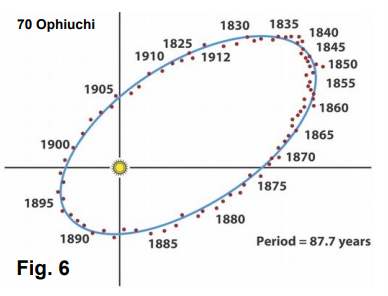
\includegraphics[width=0.5\textwidth]{imagenes/fig 6.png}
            \caption{Órbita de una binaria visual.}
            \label{fig:fig6}
        \end{figure}                
    
    En este caso el centro de masa se encuentra en $M_1a_1 = M_2a_2, a = a_1 + a_2$ siendo el semieje mayor de la masa reducida $\mu = M_1M_2 / (M_1 + M_2)$. Sin embargo, no se mide $a_i$ directamente, sino la separación angular $\alpha_i \approx d*a_i$, donde $d$ es la distancia de la estrella. Considerando también que el plano orbital de los componentes no se encuentra perpendicular a la línea de visión, sino se ve inclinado de $i$ (Fig.7), tenemos:
    \begin{align}
        M_1 + M_2 &= \frac{4 \pi^2}{G}\left(\frac{d}{\cos(i)}\right)^3 \frac{(\alpha_1 + \alpha_2)^3}{P^2} \\ 
        \intertext{Entonces}
        M_{1,2} &= \frac{4 \pi^2}{G}\left(\frac{d}{\cos(i)}\right)^3 \frac{(\alpha_1 + \alpha_2)^3}{P^2} \alpha_{1,2}
    \end{align}
    
    \item Las \textbf{binarias espectroscópicas} son sistemas no resueltos, donde el movimiento de los componentes se detecta por el \textbf{desplazamiento Doppler} de líneas de absorción en el espectro medio del sistema (Fig. 7). La velocidad radial (es decir, medida a lo largo de la línea de visión) es dada por:
    \begin{align}
    v_r &= v\sin(i) = c\delta\lambda/\lambda_0 \\
    \intertext{donde $\lambda_0$ es la longitud de onda en reposo. Visto que $Pv_i = 2\pi a_i$ tenemos}
    v_{r,2}/v_{r,1} &= a_2/a_1 = M_1/M_2 \\
    \intertext{y $a = a_1 + a_2 = P(v_1+v_2)/2\pi$, que da}
    M_1 + M_2 &= \frac{P}{2\pi G}\frac{(v_{r,1}+v_{r,2})^3}{\sin^3 i}
    \end{align}
    Por la ley de Kepler. Este método proporciona solo límites inferiores ($M_1\sin^3i$), a menos que se conozca la inclinación $i$ (p. ej. para binarias eclipsantes $i \approx 90^\circ$)   
    
    \begin{figure}[H]
        \centering
        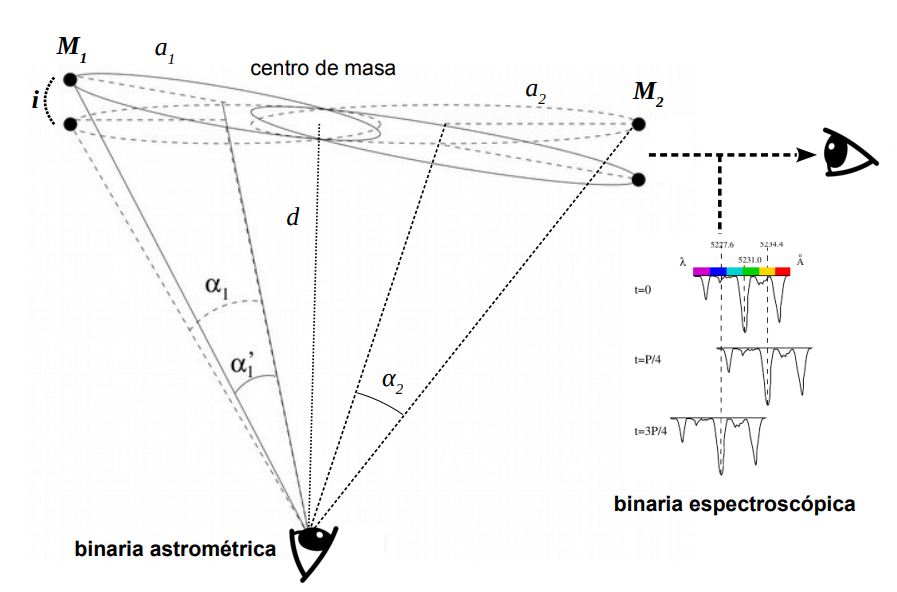
\includegraphics[width=0.5\textwidth]{imagenes/fig 7.png}
        \caption{Binaria espectroscópica.}
        \label{fig:fig7}
    \end{figure}

    \item Es muy difícil medir directamente el radio de una estrella, debido a la resolución limitada de los telescopios: $\phi = 1.2\lambda/D \approx 0,1''\lambda/400nm/(D/1m)$, la turbulencia atmosférica limitándola aún más a $\phi \ge 0.5''$ en la mayoría de los casos. En sitio, los radios estelares se pueden medir mediante \textbf{ocultaciones}, por la Luna (ocultaciones lunares) o en \textbf{binarias eclipsantes} (es decir, binarias cuyo plano orbital es paralelo a la línea de visión). En este caso (Fig 8), tenemos 
    \begin{align}
        \frac{t_4 - t_1}{P} &= \frac{2(R_1+R_2)}{l} \\
        \intertext{y}
        \frac{t_2 - t_1}{P} &= \frac{2(R_1 - R_2)}{l} \\
        \intertext{donde $l = vP$ y $P$ es el periodo orbital}  
    \end{align}

    \begin{figure}[H]
        \centering
        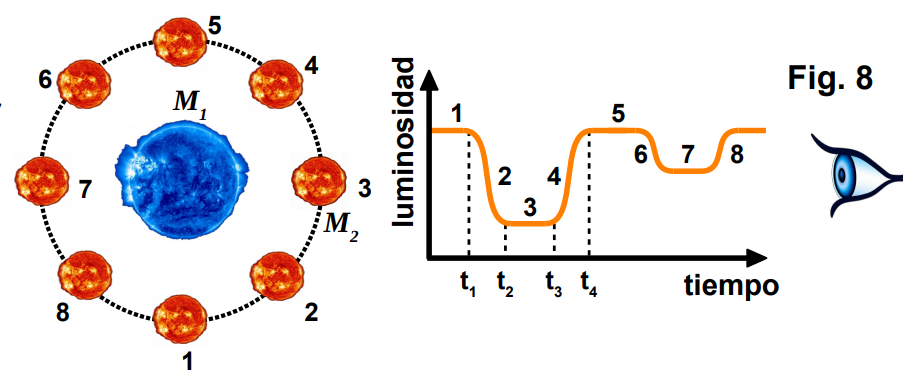
\includegraphics[width=0.5\textwidth]{imagenes/fig 8.png}
        \caption{Binaria eclipsante.}
        \label{fig:fig8}
    \end{figure}

    Los radios estelares se pueden también medir por \textbf{interferometría}: para dos telescopios situados a distancia $d_0$, la combinación de sus frentes de onda produce un patrón de interferencia con máximas de $\phi_{max,n} = n\lambda/d_0$ y mínimas de $\phi_{min,n} = (n + \frac{1}{2})\frac{\lambda}{d_0}$.
    Para dos fuentes puntuales separadas por una distancia angular $\gamma$, los extremos están también a $\gamma$. El patrón desaparece cuando los mínimos y máximos se superponen en $\gamma = \frac{\lambda}{2d_0}$. En este contexto, un disco de diámetro $D$ se comporta como dos fuentes puntuales separadas por $0.41D$ y se puede entonces resolver en un interferómetro cuando $\gamma = \frac{1.22\lambda}{d_0}$.

    \begin{figure}[H]
        \centering
        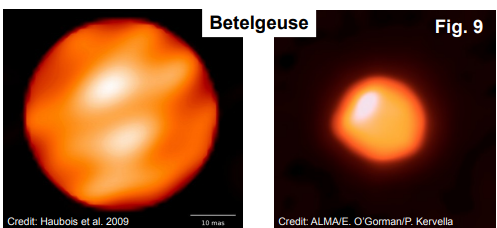
\includegraphics[width=0.5\textwidth]{imagenes/fig 9.png}
        \caption{Interferometría estelar.}
        \label{fig:fig9}
    \end{figure}

    Aunque el diámetro de la estrella gigante Betelgeuse (Fig. 9) se midió de esta manera ya en 1920, el desarrollo de la imaginería interferométrica a longitudes de onda visibles es relativamente reciente. Sin embargo, la interferometría siendo más fácil en el radio, observatorios de radio interferométricos han estado operando desde los años 1960.

    A partir de estos observables, se pueden derivar algunas \textbf{relaciones empíricas.} Las más importantes son:
    
    \subsubsection{El diagrama de Hertzsprung-Russell}    
    El diagrama de Hertzsprung-Russell (1910) relaciona la luminosidad y la temperatura efectiva de las estrellas y es el diagrama principal de la astronomía estelar (Fig. 10). En este se destacan 5 clases de luminosidad:
        \begin{itemize}
            \item Estrellas supergigantes 
            \item Estrellas gigantes luminosas
            \item Estrellas gigantes normales
            \item Estrellas subgigantes
            \item Estrellas de secuencia principal (90\% de las estrellas) 
        \end{itemize}
    \begin{figure}[H]
        \centering
        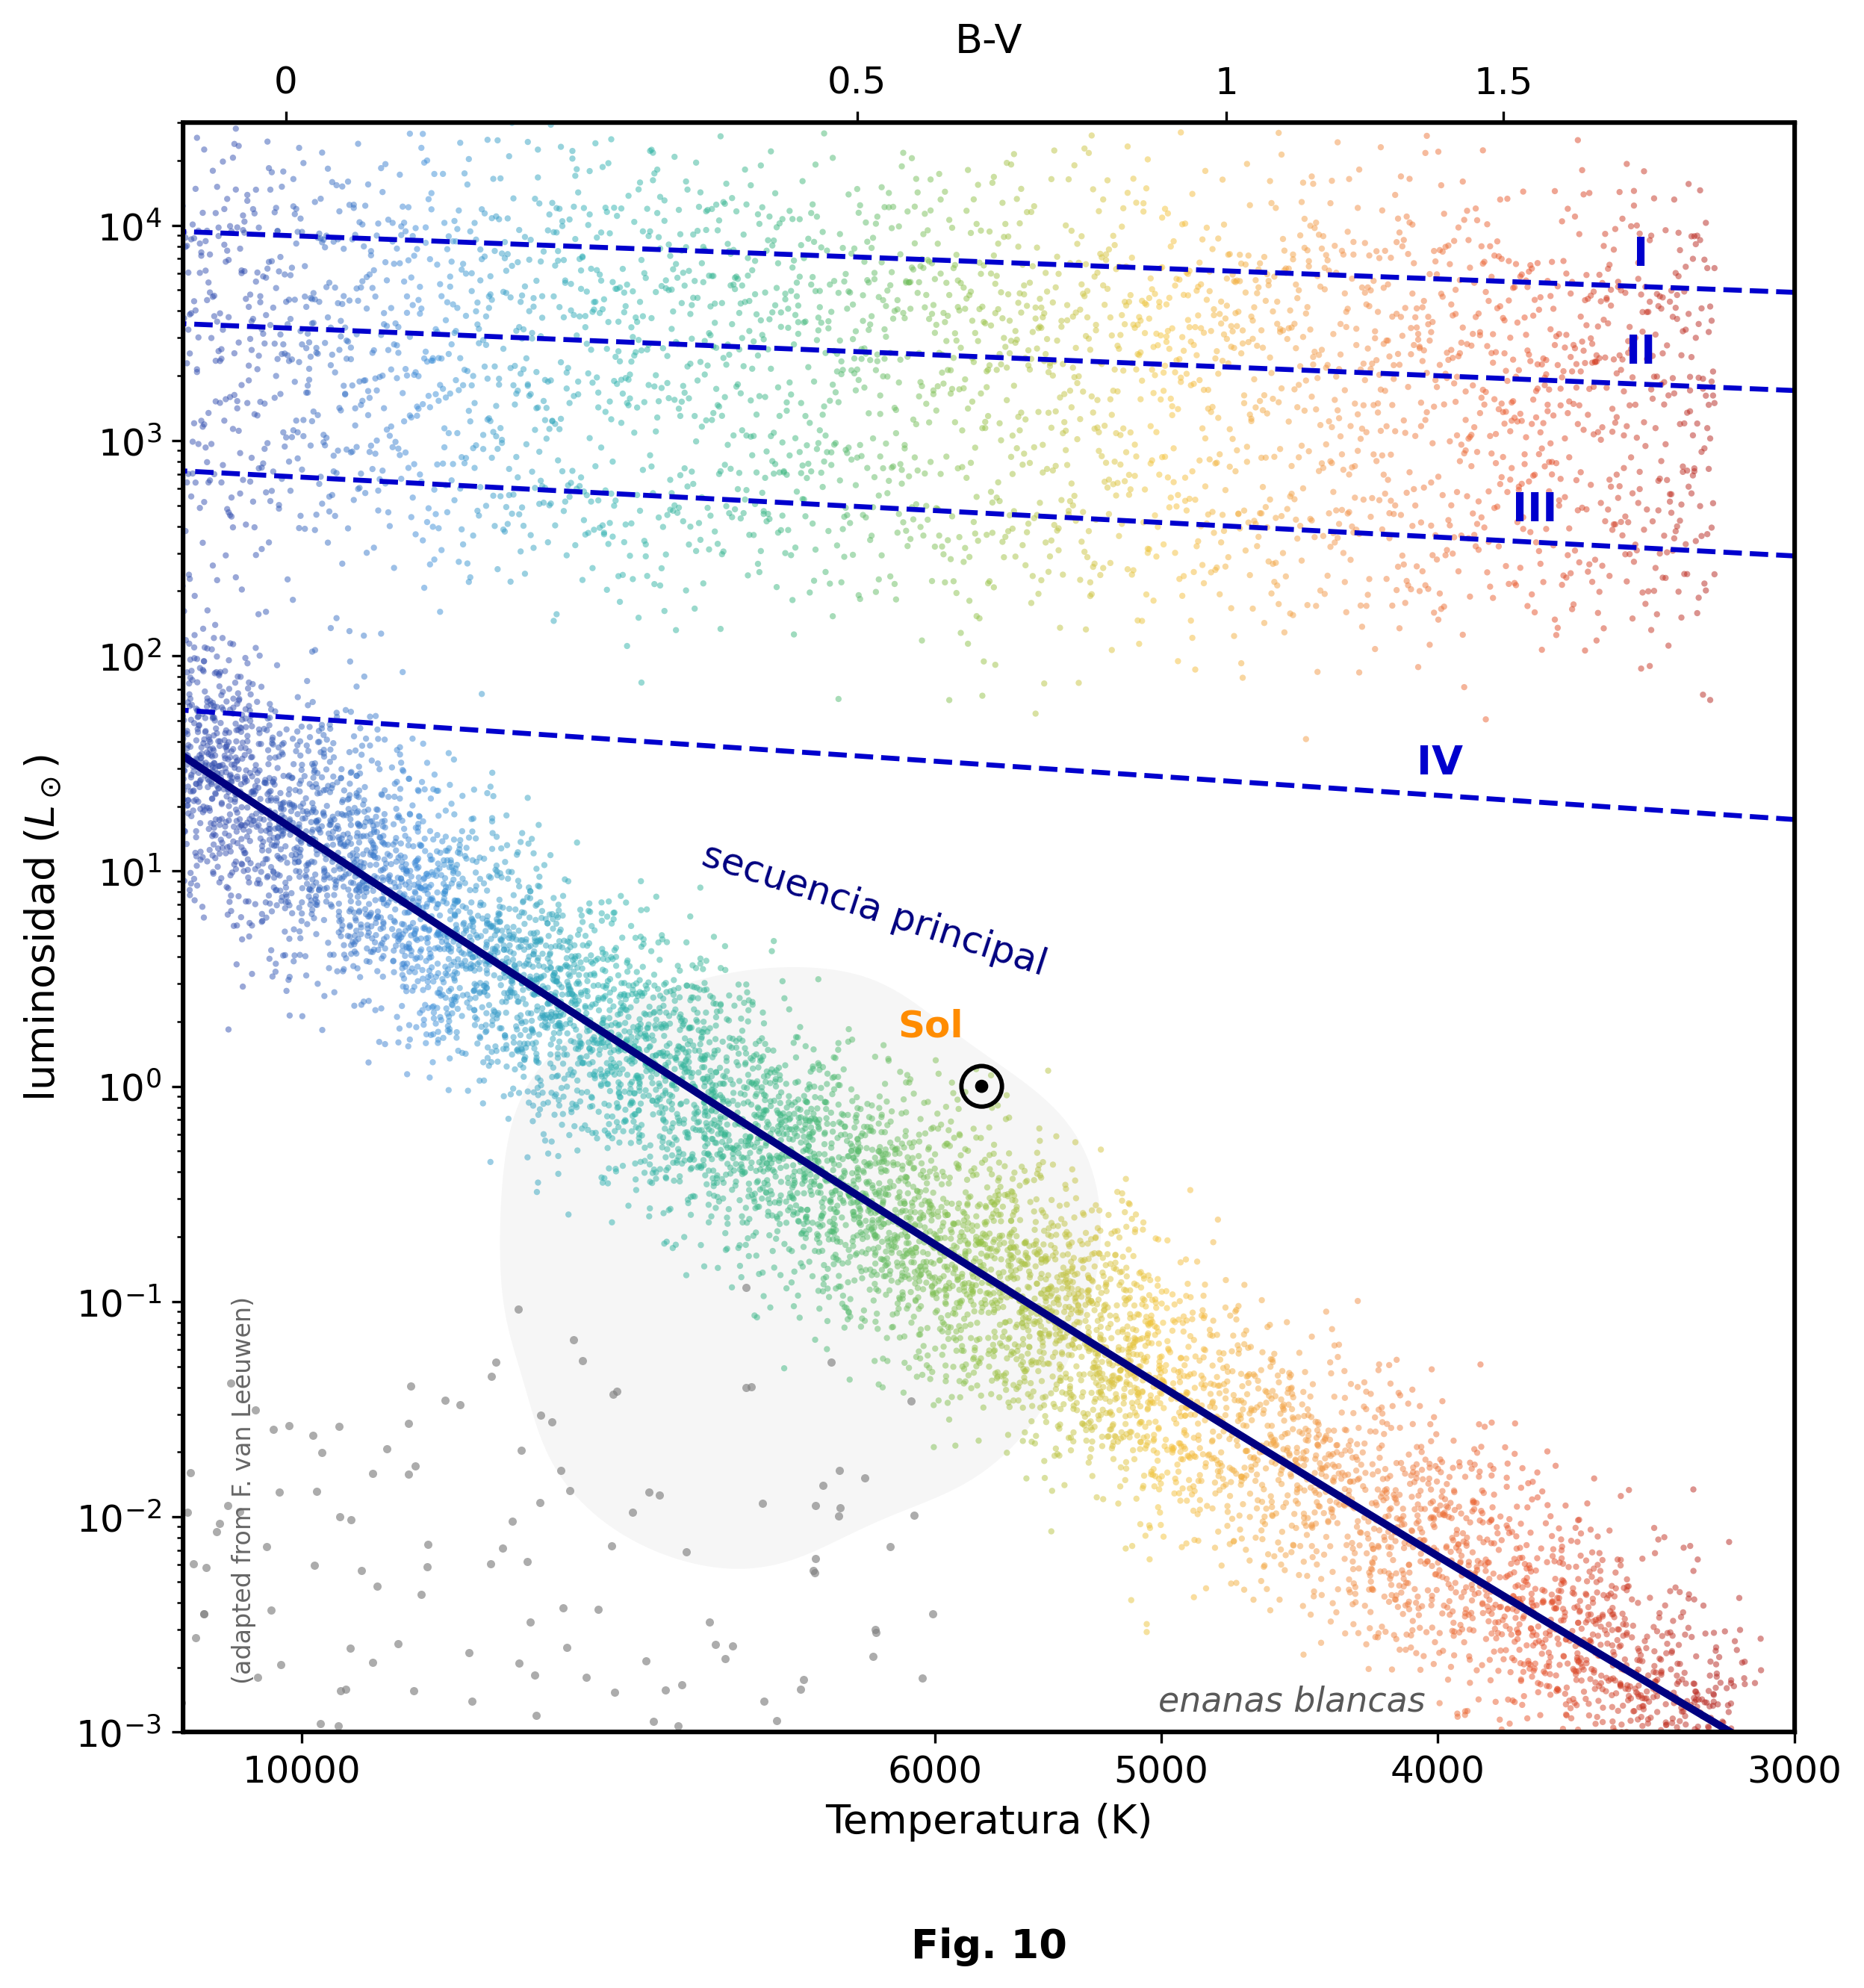
\includegraphics[width=0.5\textwidth]{imagenes/fig 10.png}
        \caption{Diagrama H-R.}
        \label{fig:fig10}
    \end{figure}

    El diagrama H.-R. permite estudiar la \textbf{evolución estelar}, así como también determinar la \textbf{edad} y la \textbf{metalicidad} de poblaciones estelares (p. ej. cúmulos estelares).

    \subsubsection{Relaciones masa-Luminosidad y masa-radio}

    Existen correlaciones entre la masa de las estrellas y ambos su luminosidad y su radio (Fig. 11). La \textbf{relación masa-luminosidad} es:
    \begin{align}
        \frac{L}{L_{\odot}} &\approx \left(\frac{M}{M_{\odot}}\right)^{4} \quad \text{para } M > 0.6M_{\odot} \\
        \intertext{y}
        \frac{L}{L_{\odot}} &\approx 0.23\left(\frac{M}{M_{\odot}}\right)^{2.3} \quad \text{para } M < 0.6M_{\odot}
    \end{align}

    \begin{figure}[H]
        \centering
        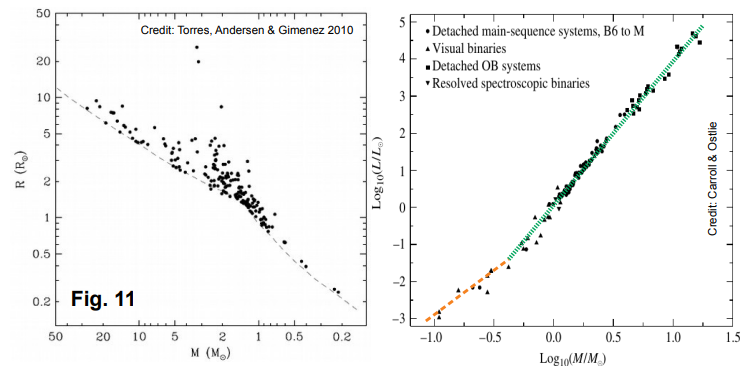
\includegraphics[width=0.8\textwidth]{imagenes/fig 11.png}
        \caption{Relaciones masa-luminosidad y masa-radio.}
        \label{fig:fig11}
    \end{figure}

    Por otra parte, la \textbf{relación masa-radio} es: $\frac{R}{R_{\odot}} \approx (\frac{M}{M_{\odot}})^{0.6}$ para estrellas de la secuencia principal. Visto que $L_S/R_S^2 \propto T_{eff}^4$, por la ley de Stefan-Boltzmann, las relaciones masa-radio-luminosidad ($L_s\propto M_S^4$ y $R_S \propto M_S^{0.6}$) dan una relación masa-temperatura de $\frac{M}{M_{\odot}}^{2.8} \approx (\frac{T}{T_{\odot}})^4$, implicando que las estrellas más masivas son también más calientes. Estas relaciones implican también que, en la secuencia principal, estrellas más calientes tienen radios más grandes. 
    
    Sin embargo, para estrellas gigantes (en el diagrama H.-R.) la relación es invertida, con temperaturas más altas indicando radios más pequeños (Tabla 1).

    \begin{center}
    \textbf{Tabla 1}\\[4pt]
    \renewcommand{\arraystretch}{1.15}
    \begin{tabular}{c|ccc}
     & \textbf{Type} & \boldmath$T_{eff}$ & \boldmath$R/R_\odot$ \\
    \hline
    \multirow{6}{*}{\rotatebox{90}{\textcolor{red}{secuencia principal}}}
     & M5V & 3100  & 0.3 \\
     & M0V & 3800  & 0.6 \\
     & G0V & 6000  & 1.1 \\
     & A0V & 10000 & 2.6 \\
     & B0V & 30000 & 7   \\
     & O5V & 45000 & 18  \\
    \hline
    \multirow{5}{*}{\rotatebox{90}{\textcolor{red}{gigantes}}}
     & M0Ia & 3700  & 500 \\
     & G0Ia & 5800  & 200 \\
     & A0Ia & 9400  & 100 \\
     & B0Ia & 27000 & 30  \\
     & O5Ia & 40000 & 25  \\
    \end{tabular}\\[4pt]
        {\footnotesize\textcolor{blue}{Credit: R. Bender}}
    \end{center}

    En resumen. La mayoría de estrellas siguen las relaciones empíricas:
    \begin{align}
        \frac{L}{L_{\odot}} &\approx \left(\frac{M}{M_{\odot}}\right)^{\alpha} \\
        \frac{R}{R_{\odot}} &\approx \left(\frac{M}{M_{\odot}}\right)^{\beta} \\
        \left(\frac{T}{T_{\odot}}\right)^4 &\approx \left(\frac{M}{M_{\odot}}\right)^{\alpha - 2\beta} \\
        \intertext{con $\alpha \approx 4$ y $\beta \approx 0.6$.}
    \end{align}

    \subsubsection{Clasificación espectral de las estrellas}
    Solemos también dividir las estrellas en tipos espectrales (OBAFGKM) en base a la intensidad de las líneas de \textbf{absorción de hidrógeno} y metales (Fig. 12). Llamada \textbf{clasificación espectral de Harvard}, fue desarrollada por Annie Jump Cannon en 1924. Cada tipo espectral se divide además en diez sub-clases (0-9). Históricamente importante, este esquema se usa hoy más como una ``taquigrafía''. Agregando la clase de luminosidad, en el esquema de Harvard nuestro Sol es de tipo G2V:
    \begin{equation}
        R_{\odot} = 109 R_{\oplus}, M_{\odot} = 333'000 M_{\oplus}, T_{eff,\odot} = 5800 K, L_{\odot} = 3.826 \times 10^{26} W
    \end{equation}

    \begin{figure}[H]
        \centering
        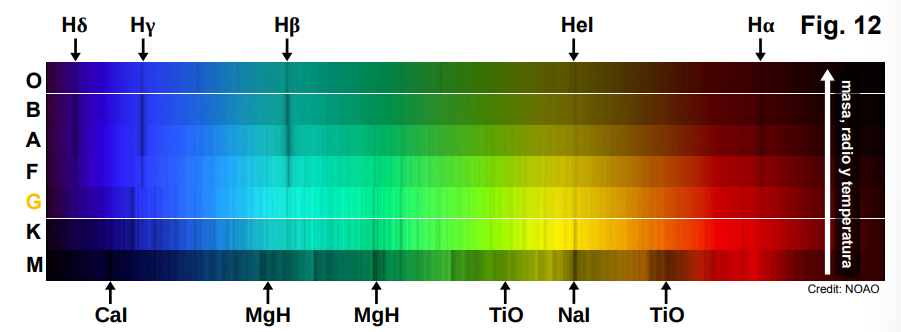
\includegraphics[width=0.8\textwidth]{imagenes/fig 12.png}
        \caption{Clasificación espectral.}
        \label{fig:fig12}
    \end{figure}

    El esquema de Harvard, como se usa hoy, está organizado para correlacionar el tipo espectral con la temperatura superficial de la estrella y, entonces, su radio y masa. Sin embargo, respecto a estas dos últimas cantidades la relación no es lineal (Fig. 13):

    \begin{figure}[H]
        \centering
        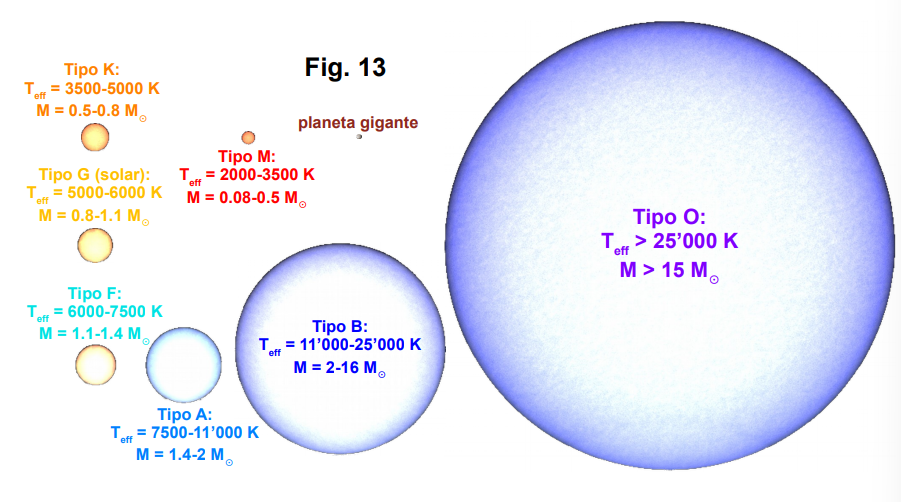
\includegraphics[width=0.8\textwidth]{imagenes/fig 13.png}
        \caption{Relación tipo espectral - radio - masa.}
        \label{fig:fig13}
    \end{figure}
    \end{itemize}
\end{enumerate}

\section{Unidad I: Ecuaciones de estructura}
\subsubsection{Suposiciones}
Las estrellas son en primera aproximación objetos astrofísicos estructuralmente simples. Sus interiores se pueden modelar analíticamente con un mínimo de suposiciones. Asumiremos que las estrellas son:
    \begin{itemize}
        \item \textbf{Esféricamente simétricas}, así que hay solo movimientos radiales.
        \item \textbf{Estacionarias} desde el punto de vista de su evolución: es decir, que esta última toma mucho más tiempo que los procesos internos. Significa que podemos suponer que sus propiedades globales no cambian con el tiempo.
        \item \textbf{Aisladas}: que su estructura depende solo de propiedades \textbf{intrínsecas}.
        \item \textbf{Químicamente homogéneas}.
    \end{itemize}
Esto es principalmente exacto para la mayoría de estrellas durante la mayor parte de su vida. Tenemos entonces que determinar los parámetros siguientes:
\begin{equation}
    M(r), \rho(r), P(r), T(r), L(r)
\end{equation} 
De \textbf{I} (simetría radial), consideramos conchas esféricas de espesor $dr$ (Fig 14) y volumen $dV = 4\pi r^2 dr$, así que
\begin{align}
    \frac{dM}{dr} &= 4\pi r^2 \rho \quad \text{relación masa-densidad}\\
    \intertext{donde $\rho$ es la densidad local del gas.}
    \intertext{Un elemento de volumen de sección transversal $\delta S$ y espesor $\delta r$ estará en equilibrio entre gravedad y presión interna (Fig. 11) si}
    (P (r + \delta r) - P(r))\delta S &+ \frac{GM(r)\rho(r)\delta S \delta r}{r^2} = 0 \\
    \intertext{así que}
    \frac{dP}{dr} &= -\frac{GM(r)\rho(r)}{r^2} \quad \text{equilibrio hidrostático} \\
    \intertext{o, usando la relación masa-densidad:}
    \frac{dP}{dr} \frac{dr}{dM} &= -\frac{GM(r)\rho (r)}{r^2} \frac{1}{4\pi r^2 \rho} = -\frac{GM(r)}{4\pi r^4} \\
\end{align} 
Estas dos primeras ecuaciones ya nos permiten estimar la presión central. Por ejemplo, el gradiente de la presión puede ser aproximado (de manera brusca) por $\frac{dP}{dr} \sim \frac{P_{surf}-P_c}{R_S} \approx -\frac{P_c}{R_S}$ en $r_{0.5}=R_S/2$, visto que $P \to 0$ en $R_S$. Si asumimos además que $M(r_{0.5}) \sim M_S/2$, tenemos $\rho_{0.5} \sim \bar{\rho} = \frac{3M_S}{4\pi R^4_S}$
y por lo tanto, $P_c \sim \frac{3G}{8\pi}\frac{M_S^2}{R_S^4}$. En el caso del sol, $P_{c,\odot} \sim 7*10^9 atm$, que es demasiado pequeño.

Por otro lado, combinando la ecuación de equilibrio hidrostático y el perfil de masa-densidad produce $\frac{d}{dr}(P+\frac{GM}{8\pi r^4}) = -\frac{GM^2}{2\pi r^5} < 0$ : el lado derecho siendo 0 en $r = 0$ dado que $M \propto r^3$, $P_c>\frac{GM^2_S}{8\pi R^4_S}$. En el caso del Sol, da $P_{c, \odot} > 4.4 \times 10^{8} atm$, que nos ayuda mucho (de hecho, \textbf{$P_{c,\odot}\approx 3.4*10^{11}$atm}).
Continuando. La aceleración de un elemento de masa $dM = \rho dr dS$ es:
\begin{align}
    \ddot{r} dM &= - \frac{GM}{r^2}dM + P(r) dS - P(r + dr)dS \\
    \intertext{con $P(r+dr) = P(r)+\frac{\partial P}{\partial r}dr$. Entonces}
    \frac{\partial ^2 r}{\partial t^2} &= -\frac{GM}{r^2} - \frac{1}{\rho}\frac{\partial P}{\partial r} = -\frac{GM}{r^2} - 4\pi r^2 \frac{\partial P}{\partial M} \quad \text{\textbf{ecuación de movimiento}} 
\end{align}  
Si $P = 0$ hay solo el término de gravedad y la estrella se derrumba: después de un tiempo $t$, se habrá contraído de $\delta r = - \frac{GM(r)t^2}{2r^2}$. El tiempo de caída libre o \textbf{tiempo dinámico}, se encuentra cuando $\delta r \sim R_S$, con 
\begin{equation}
    t_{dyn} \sim \sqrt{\frac{2R_S^3}{GM_S}} = \sqrt{\frac{3}{2\pi G \bar{\rho}}}
\end{equation}

Para el sol el tiempo dinámico es aproximadamente 40 minutos, es decir, 14 órdenes de magnitud menos que su edad ($\sim 4.6$ Ga). Eso implica que:
    \begin{itemize}
        \item Cualquier \textbf{salida del equilibrio} será \textbf{inmediatamente observable}.
        \item El equilibrio hidrostático tiene que ser \textbf{restaurado rápidamente}.
        \item En caso de oscilaciones, su periodo será proporcional a la densidad.
        \item Por lo tanto, estrellas están muy cerca del \textbf{equilibrio hidrostático}
    \end{itemize}
Esto valida también la suposición II.
\subsubsection{Teorema del virial y ecuación de estado}
Agregando el elemento de volumen a la ecuación de equilibrio hidrostático se obtiene:
\begin{align}
    \frac{4}{3} \pi r^3 dP &= -\frac{4}{3}\pi r^3 \frac{GM(r)\rho (r)}{r^2}dr = -4\pi r^2 \frac{GM}{r} \rho dr \\
    \intertext{Integramos por partes del lado izquierdo}
    4\pi [r^3P]_{r=0, P = P_c}^{r=R_s, P = P_s} &-3 \int _0^{R_s} P4\pi r^2 dr \\
    \intertext{lleva a}
    \int _0 ^{R_S} 3P4 \pi r^2 dr &= \int _0 ^{R_S} \frac{GM}{r} 4 \pi r^2 \rho dr \\
    \intertext{o}
    3 \int _0 ^{V_S} PdV &= -E_g
\end{align}

Donde $E_g$ es la energía gravitacional. Esta es la forma general del teorema de virial. Consecuentemente, la presión necesaria para sostener una estrella es $-E_g/3V$.
Asumiendo que esta se compone de un gas ideal \textbf{monoatómico} con ecuación de estado:

\begin{equation}
    P(\rho , T) = \frac{k}{\mu m_H} \rho T
\end{equation}
Donde $\mu$ es la masa promedio de una partícula de gas en unidades atómicas, la energía cinética de las partículas de gas por unidad de masa es

\begin{align}
    u &= \frac{3}{2} \frac{kT}{\mu m_H} = \frac{3}{2} \frac{P}{\rho} \\
    \intertext{y la energía cinética total $U = \int udm$.}
    \intertext{Recordando que $dV = dm/ \rho $ el teorema del virial se vuelve $U = -\frac{1}{2}E_g$.}
\end{align}

Visto que la energía gravitacional aumenta cuando el radio disminuye, contracciones que mantienen el equilibrio hidrostático aumenta ambos $P$ y $T$. A la inversa, un aumento de la presión/temperatura interna causará una expansión y enfriamiento del núcleo estelar (retroalimentación negativa).

La masa molecular media del gas depende de su composición y estado con $\mu = 1$ para H neutro y $\mu = 0.5$ para H ionizado. En este caso, tenemos para hidrógeno $1e^-$, para helio $2e^-$ y para metales $\sim A/2 e^-$. Por lo tanto, las densidades numéricas se pueden escribir (tabla 1):

\begin{table}[H]
\centering
\renewcommand{\arraystretch}{1.5} % Aumenta un poco la altura de las filas para que respire el texto
\begin{tabular}{|l|c|c|c|}
\hline
\textbf{Tabla 1} & \textbf{H} & \textbf{He} & \textbf{metales} \\ \hline
núcleos & \(X\rho/m_h\) & \(Y\rho/4m_h\) & \(Z\rho/Am_h\) \\ \hline
electrones & \(X\rho/m_h\) & \(2Y\rho/4m_h\) & \(\approx Z\rho 2/Am_h\) \\ \hline
\end{tabular}
\end{table}

Donde las abundancias de los elementos por unidad de masa son \textbf{X} para hidrógeno $(m_H + 1e^-)$, \textbf{Y} para helio $(4m_H + 1e^-)$ y \textbf{Z} para el resto (metales: $Am_H + \sim A/2e^-$), con $X+Y+Z = 1$ por definición. Por lo tanto $Z$ se llama \textbf{metalicidad}. En el caso del sistema solar, $Z_\odot \approx 0.02$, mientras las abundancias primordiales son $X\approx 0.75$ y $Y \approx 0.25$.

\begin{align}
    \intertext{Si $A \gg 1$ }
    n &= \frac{\rho}{m_H} \left(2X + \frac{3}{4} Y + 2Z\right) = \frac{\rho}{\mu m_H} \\
    \intertext{entonces}
    \mu &= \left(2X + \frac{3}{4}Y + 2Z\right)^{-1}
\end{align}

\subsubsection{Energía interna y escalas de tiempo}

Las estrellas pierden energía por radiación y por lo tanto, requieren una fuente de energía interna para evitar el colapso. En caso de un gas ideal, la energía (gravitacional) total disponible es $\sim GM_S^2/2R_S$. Asumiendo que esta energía potencial se convierte en radiación con tasa constante, la escala de tiempo térmica (o de Kelvin-Helmholtz) es $t_{th} \sim \frac{GM_S ^2}{2R_S L_S}$. 
Para el sol, se tiene $t_{th, \odot} \sim 1.5*10^7$ años. Sin embargo, sabemos que su luminosidad no cambió mucho durante los últimos $10^9$ años. Cabe también señalar que las reacciones químicas llevan menos energía, siendo limitadas a $\sim 10^4$ W/g (o 10'000 años en el caso del Sol).

Esto fue un problema para los físicos del siglo XIX:

\begin{quote}
    \itshape
    ``We may, therefore, accept, as a lowest estimate for the sun's initial heat, 10,000,000 times a year's supply at the present rate, but 50,000,000 or 100,000,000 as possible, in consequence of the sun's greater density in his central parts.''
    \upshape
    \par\vspace{0.5em}
    \raggedleft
    - William Thomson (Lord Kelvin), 1862
\end{quote}


\section{Ecuaciones de estructura}

perfil de masa

\begin{equation}
    \frac{dM}{dr} = 4\pi r^2 \rho
\end{equation}

equilibrio hidrostático

\begin{equation}
    \frac{dP}{dr} = -\frac{GM\rho}{r^2}
\end{equation}

perfil de luminosidad

\begin{equation}
    \frac{dL}{dr} = 4\pi r^2 \rho \epsilon
\end{equation}

radiativo

\begin{equation}
    \frac{dT}{dr} = -\frac{3\kappa \rho L}{16\pi a c T^3 r^2}
\end{equation}

convectivo

\begin{equation}
    \frac{-\mu m g}{R_b}\left(1 - \frac{1}{\gamma (\rho , T)}\right)
\end{equation}

\begin{equation}
    P = \frac{\rho k T}{\mu m}
\end{equation}

gráfico inestable

\begin{equation}
    Luminosidad \propto \frac{1}{k}\left(\frac{\gamma - 1}{\gamma}\right)
\end{equation}

gráfico feo radiación superficies masa 


\subsection{Soluciones}
\begin{itemize}
    \item Politropes
    \begin{equation}
        P = C \rho^{\gamma}
    \end{equation}
    
    \begin{equation}
        \gamma = 1 + \frac{1}{n}
    \end{equation}

    $n:$ Índice politrópico.

    Para $n = 3/2$ estrellas convectivas materia degenerada no relativista.
    
    Para $n = 3$ sistema dominado por radiación materia degenerada relativista.
    \item Ansatz $\rho (r) = \rho_c e ^{r/H}$ con $H = \delta R_s$, $\delta \sim 0.1$ y $\rho_c \sim 230g/cm^3$ 
    \item 
    
    
    
\end{itemize}

\end{document}